
% \pagenumbering{arabic}
% \setcounter{page}{1}


\chapter{Background} \label{sec:background}


In this chapter, we explain the basic concepts required for comprehending this dissertation.



\section{Blockchain}
Public blockchains are the most promising underlying technology for many applications. They are aiming to be decentralized, transparent, and immutable. However, they are also slow, expensive, and have limited functionality. They can and will replace many intermediary entities we know of today. However as we will dive deeper in this subject, blockchain, as a technology is in its infancy. The public aspect of these blockchains changes many assumptions developers and system designers have about the data flow within their applications. 

Blockchain works by having a decentralized network of nodes that are incentivized to maintain the network. The nodes are incentivized by receiving rewards in the form of cryptocurrency. The nodes are also responsible for verifying the transactions and adding them to the blockchain. The blockchain is a chain of blocks, each block containing a list of transactions. The order of the transactions in each block is important as it indicates the order of events in the blockchain.


\begin{figure}[h]
    \centering
    {\caption{The building blocks of blockchain technology~\cite{gaggioli2019middleman}}}
    {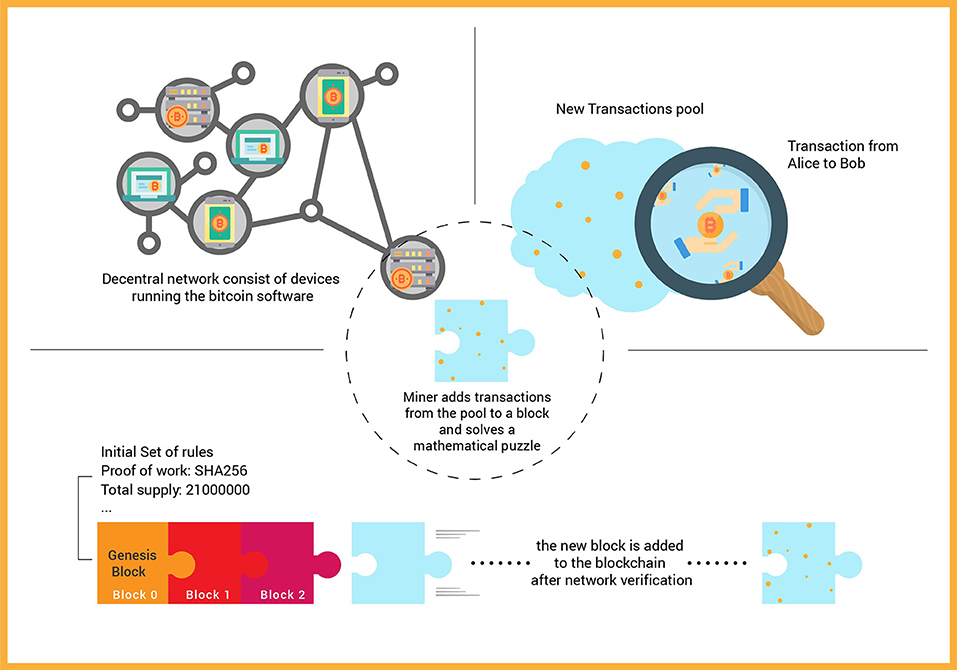
\includegraphics[width=0.8\textwidth]{figures/blockchain-buildingblocks.jpg}}
    \end{figure}
    %https://www.lucidchart.com/invitations/accept/f8ca2662-5269-425d-9deb-deb14af2aac7


This technology has the potential of many interesting applications, from digital cash (\eg Bitcoin~\cite{nakamoto2008bitcoin}), prediction markets~\cite{clark2014decentralizing}, and decentral governance~\cite{aragonwebsite}. Bitcoin, started in 2009, was the first application of blockchain technology and since then the concept of decentral ledger has grown to many other applications that just a ledger holding transaction data. 


\section{Ethereum}

Ethereum~\cite{wood2014ethereum} is a prominent public blockchain that has attracted the largest developer headcount compared to other blockchains. It is an extension of its predecessor, Bitcoin~\cite{nakamoto2008bitcoin}, but with significant enhancements, notably the addition of \textit{smart contracts}. These smart contracts are applications residing on the blockchain that can immutably execute their verified code. Ethereum operates on a Turing-complete virtual machine, the \texttt{Ethereum Virtual Machine (EVM)}, allowing programs to live and be executed on the blockchain. This differs from Bitcoin's UTXO\footnote{Unspend Transaction Output} model, which primarily supports value transfers and has a scripting language for extending transaction functionality to a limited extent. In contrast, Ethereum's Turing-complete language opens up limitless possibilities.  All transactions and executions on Ethereum are verified by a decentralized network of nodes. The nodes are incentivized to verify transactions and execute smart contracts by receiving rewards in the form of Ether, the native cryptocurrency of Ethereum. 

Ethereum blockchain started in 2015 using the similar consensus mechanism as Bitcoin, called Proof of Work (PoW), also known as mining. However, in 2020, Ethereum started the transition to Proof of Stake (PoS) consensus mechanism. The main difference between PoW and PoS is that in PoW, the nodes are incentivized to solve a computationally hard puzzle to be able to add a block to the blockchain. However, in PoS, the nodes are incentivized to stake their Ether to be able to add a block to the blockchain. The PoS mechanism is more energy efficient and more scalable than PoW. Ethereum fully switched to PoS in September 2022 in an event called the \textit{Merge}, and reduced its energy consumption by 99.5\%~\cite{themerge}. In this dissertation, we do not directly focus on the consensus mechanisms, however, we will discuss the implications of the consensus mechanism on the blockchain security in chapter ~\ref{sec:frontrunning}. 


\subsection{Smart Contracts}
Smart contracts are small codebases (applications) that live on a blockchain. The technical details of smart contracts are not necessary to understand for this report. In short, Smart contracts, developed using Solidity as the main high-level programming language, are compact code bases on the blockchain. They can be viewed as blackbox applications receiving user inputs, following a code flow to produce outputs that can update the contract's state and trigger monetary transactions. Smart contracts, mostly has been used for tokenized economy, except some technical limitation, the functionalities are limitless. From unstoppable gambling games to complete voting and payroll systems. 

However, as noted earlier, everything on a blockchain is compromised of transactions and blocks. The order of the transactions in each block indicates the order of events in the Ethereum blockchain. Given that miners, and recently entities named \textit{block builders}, are in control of the order, it is possible for these entities to reorder the transaction in a block, or even not include a transaction in a block for higher financial gain from the new order. This is the basics of blockchain front-running that we discuss in the next chapters. 


\subsection{Ethereum Network}
The peer to peer aspect of Ethereum network enables the possibility for a full decentralized network. As the vision of Ethereum is a world computer that everyone can use, the network is designed to be accessible to everyone. This means that anyone can run a full node and be part of the network. The network is designed to be trustless, meaning that the nodes do not need to trust each other. The network is also permissionless, meaning that anyone can join the network and be part of the consensus. This is in contrast to the traditional financial systems that are centralized and permissioned, meaning that only a few entities are in control of the network and the information flow.


\subsection{mempool}
When a user sends a transaction to the Ethereum network, one node will validate the transaction and propagate it through the network. While this transaction is still not included in the block, it is stored in the memory of all the nodes, also known as \textit{mempool}. The mempool is a list of the transactions that are not yet included in the blockchain, however the order of the transactions are different for each node, as they have received the transactions in different order. This opens up the block builder to the possibility of reordering the transactions in the block they build for their own financial gain.


